% !TeX root = ../relazione.tex

\chapter{Il formato dei database file}

A differenza di molti altri motori di database SQL, un database SQLite memorizza tutto all’interno di un singolo file chiamato \textbf{main database file}. 

Il formato dei file SQLite è stabile, retrocompatibile con le versioni precedenti e multipiattaforma, infatti, è possibile copiare lo stesso file su sistemi a 32 e 64 bit o su architetture in cui l’ordine dei byte è di tipo big-endian o little-endian.

I file dei database SQLite sono raccomandati dall’US Library of Congress \cite{uslibraryofcongress}, in quanto il formato massimizza la sopravvivenza e l’accessibilità dei contenuti digitali.

\section{I file Hot Journals}
Con il termine Hot Journals si intendono quei file che contengono le informazioni necessarie per poter ripristinare il database ad uno stato consistente.
SQLite utilizza un secondo file chiamato “rollback journal” o, se l’opzione WAL è disponibile, un file chiamato “Write-Ahead Log”.
In questi file verranno conservate informazioni aggiuntive relative alle transazioni eseguite, che in caso di interruzione del sistema, prima del completamento di una transazione, consentiranno di ripristinare il database ad uno stato consistente eseguendo il rollback di tutte le operazioni eseguite fino al commit precedente.


\section{Pagine}
Un file SQLite è suddiviso in pagine della stessa dimensione. La dimensione in byte di una pagina è compresa da un minimo di 512 byte a un massimo di 65536 byte. 

Ciascuna pagina ha una propria intestazione, la quale permette di ottenere diverse informazioni sulla pagina in cui è situata. 

Il numero massimo di pagine ammonta a ($2^{32}$ – 2), le pagine sono numerate a partire da uno e ciascuna pagina può essere di un determinato tipo a seconda della funzione ricoperta.

\newpage

\section{Header del database}
L’header di un database SQLite consente di determinare le informazioni essenziali per poter operare su questi tipi di file. È collocata nei primi 100 byte del main file e consiste di 32 campi. Le informazioni sono immagazzinate seguendo l’ordine dei byte big-endian.

\medskip
Ad esempio, all’offset 0 leggendo 16 byte si potrà trovare il “Magic Header”, che altro non è che una stringa che identifica che il file è di tipo SQLite.

\medskip

Di seguito è presente una tabella che riassume i campi presenti nell’header:
\begin{figure}[ht]
	\centering
	\caption{Il formato dell'header del database}
	\label{fig:sqlitedatabaseheader}
	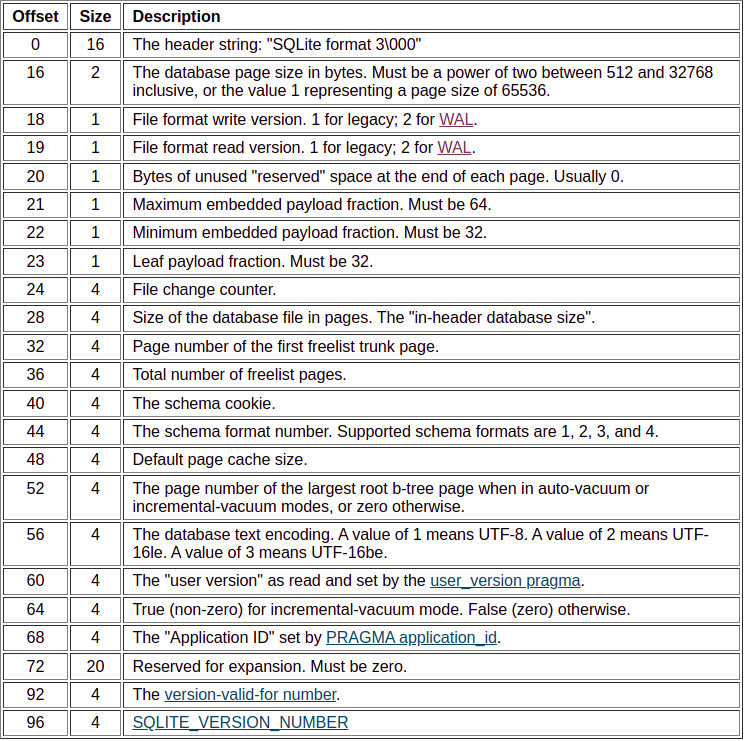
\includegraphics[scale=0.5]{assets/database_header_sqlite}
\end{figure}

\newpage

\section{Freelist}

In ogni istante di tempo un database SQLite potrà avere un certo numero di pagine attive e di pagine non attive. Quelle attive conterranno dei dati validi per il database, mentre, le pagine non attive conterranno dati che non sono più ritenuti validi per la base di dati.
Una pagina diventerà inattiva, quando arriverà a contenere solo informazioni non più valide. 

Le pagine non utilizzate (inattive) verranno memorizzate in delle freelist, che consentiranno di poterle riutilizzare non appena ci saranno ulteriori informazioni da memorizzare.

La freelist è una struttura dinamica organizzata come una lista concatenata, ciascun elemento ha una dimensione di 4 byte seguenti l’ordine dei byte big-endian. Ogni elemento della lista consiste di due interi da 2 byte ciascuno, il primo intero è il numero della seguente pagina non attiva nella freelist, mentre, il secondo intero è il numero di inserimenti all’interno di quella pagina. Per segnalare il termine degli elementi nella freelist, SQLite memorizzerà nell’ultimo elemento della lista il valore 0 per identificarne il termine.
All’interno dell’header del database sono presenti delle informazioni utili per operare con le freelist;
\begin{itemize}
\item All'offset 36 è presente un intero di 4 byte, che rappresenta il numero delle pagine nella freelist
\item All’offset 32 è presente il numero della prima pagina all’interno della freelist
\end{itemize}


\section{Le pagine di tipo b-tree}

SQLite utilizza come algoritmo per memorizzare le informazioni il b-tree. Questo algoritmo ci consente di memorizzare le informazioni come coppie di chiave:valori.

\medskip

Ciascuna pagina b-tree è di uno dei seguenti tipi;
\begin{itemize}
\item interna di tipo indice
\item interna di tipo tabella
\item foglia di tipo indice
\item foglia di tipo tabella
\end{itemize}

Le pagine foglie contengono le chiavi e, nel caso in cui la pagina sia di tipo tabella, conterranno anche i dati associati alle chiavi. Mentre, per quanto riguarda le pagine interne, esse conterranno solamente le chiavi e per ogni chiave il puntatore associato alla pagina figlia.

\newpage
	
\subsection{Struttura}

Ogni pagina è suddivisa nelle seguenti sezioni ordinate;

\begin{figure}[ht]
	\centerline{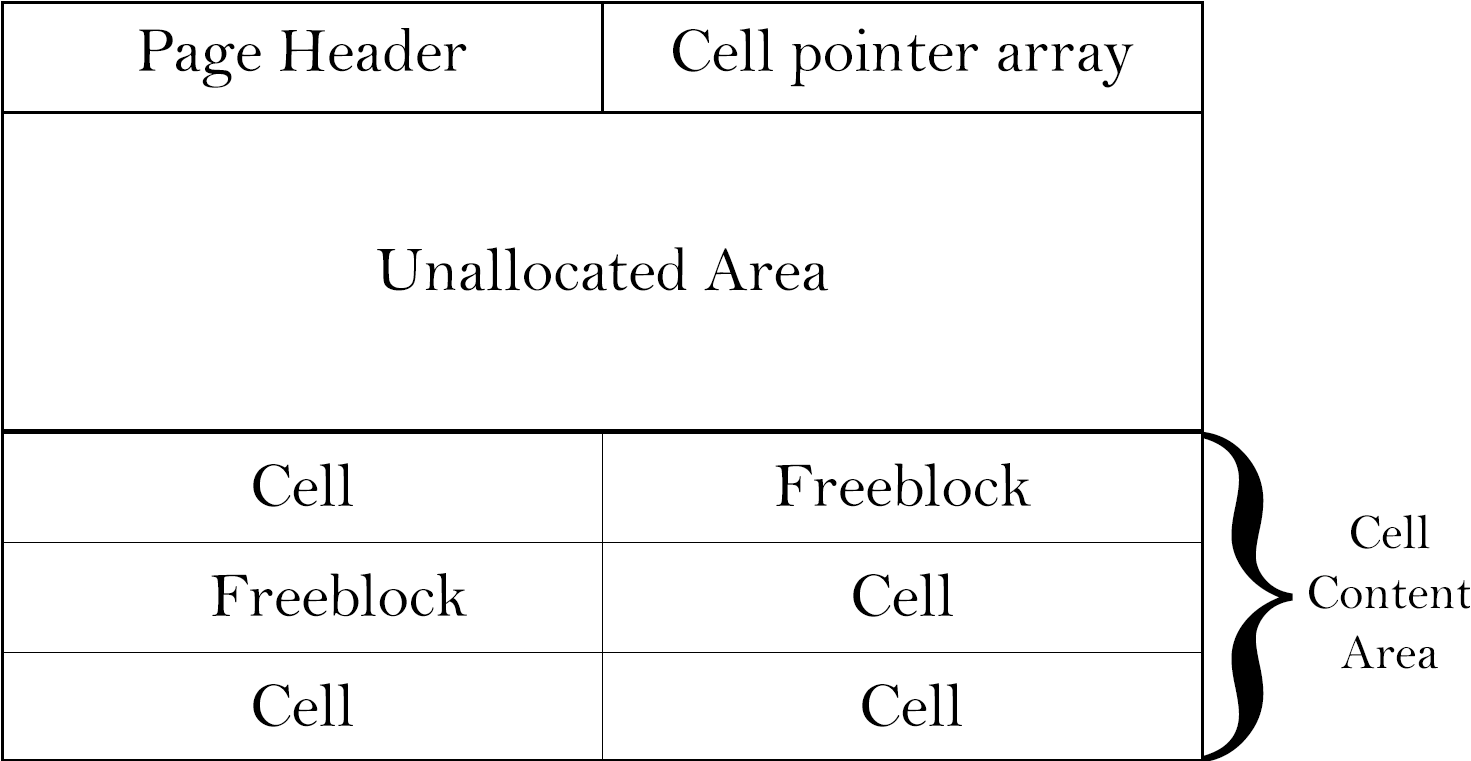
\includegraphics[scale=0.25, ]{assets/b-tree-page-structure}}
	\caption{La struttura di una pagina b-tree}
	\label{fig:btreepagestructure}
	
\end{figure}

\begin{itemize}
\item I primi 100 byte rappresentano l’header del database (ciò vale solo per la prima pagina), questa sezione non è rappresentata nella figura precedente
\item Verranno utilizzati dagli 8 ai 12 byte per rappresentare l’header della pagina
(8 byte per le pagine foglie e 12 per le pagine interne)
\item Un array che contenente i puntatori alle celle
\item L’area contenente lo spazio non allocato presente all’interno della pagina
\item L’area contenente il contenuto delle celle
\item L’area riservata
\end{itemize}

L’array contenente i puntatori alle celle userà un numero di byte pari al numero di celle puntate per 2 byte (ciascun elemento dell’array rappresenterà l’offset al contenuto della cella dall'inizio della pagina).

L’area non allocata contiene dei byte che non sono utilizzati, ma che potranno permettere all’area contenente il contenuto delle celle di espandersi. Quest’area non appena il database sarà costruito verrà inizializzata a 0. 

L’area riservata può essere utilizzata dalle estensioni di SQLite per fornire funzioni aggiuntive, come l’estensione SQLite Encryption Extension (SEE), la quale permette ad un applicazione di scrivere e leggere su database cifrati.

\newpage

\subsection{Il formato dell’header}

Come già detto in precedenza, l’header della pagina potrà occupare 8 o 12 byte, a seconda del tipo.

\medskip

Di seguito ne viene riportata la struttura;

\begin{itemize}
\item Il primo byte dell’header indicherà il tipo di pagina b-tree
\SubItem{Il valore 2 (0x02) indica una pagina interna di tipo indice}
\SubItem{Il valore 5 (0x05) indica una pagina interna di tipo tabella}
\SubItem{Il valore 10 (0x0a) indica una pagina foglia di tipo indice}
\SubItem{Il valore 13 (0x0d) indica una pagina foglia di tipo tabella}

\item I successivi due byte indicano l’inizio del primo freeblock nella pagina, o 0 se quest'ultimo non è presente
\item Il quarto e il quinto byte rappresentano un valore intero indicante il numero di celle nella pagina, con il termine di cella si fa riferimento a un record.
\item Nei successivi due byte troviamo l’offset dall’inizio della pagina all’inizio dell’area contenente le celle.
\item Nel byte successivo è memorizzato il numero dei byte liberi frammentati all’interno dell’area contenente le celle.
\item Nelle pagine interne ci saranno 4 ulteriori byte per conservare il puntatore più a destra che permette di trovare la cella con la chiave più grande.
\end{itemize}

\subsection{Freeblock}
I freeblock sono strutture dati utilizzate da SQLite per identificare lo spazio non utilizzato all'interno dell'area contenente le celle di ciascuna pagina.
Queste aree vengono memorizzate per permettere a SQLite di poterle riutilizzare. 
Come illustrato in precedenza, all'interno dell'header della pagina c'è un campo che sta a indicare l'offset dall'inizio della pagina al primo freeblock.
I freeblock sono organizzati come una catena, infatti, ciascun elemento è composto da 4 byte; i primi due identificano l'offset al prossimo freeblock e i successivi due la grandezza del freeblock in byte.
Se la grandezza del freeblock dovesse essere uguale a 0 allora ciò indicherebbe che non sono presenti ulteriori freeblock nella pagina.

\newpage

%\subsection{Spazio non allocato}
%a

%\subsection{Area contenente le celle}
%a

%\subsection{Area riservata}
%a

\section{Tipi di dati}
Prima di poter illustrare il formato dei record, è necessario spiegare due tipi di dati, che vengono utilizzati da SQLite per codificare le informazioni dei record.

\paragraph{Il tipo di dato varint}
\hfill \break
SQLite fa un ampio uso delle variabili varint (Variabile-Length Integers), esse permettono di rappresentare interi senza segno e hanno una lunghezza che può variare da 1 byte ai 9 byte. Questo tipo di dato gode delle seguenti proprietà;

\begin{itemize}
\item Rappresentare interi piccoli utilizzando meno byte
\item Conoscere la lunghezza in byte della variabile guardando il primo byte
\item Avere l'ordine lessicografico e numerico identico, ciò permette di poter utilizzare queste variabili come chiavi. 
\end{itemize}


\paragraph{I codici serial types}
\hfill \break
Sulla base dei valori rappresentati dalle variabili spiegate in precedenza, all'occorrenza, ovvero nel momento in cui andremo a identificare i campi da cui è composto un record, SQLite utilizza i serial types per codificare il tipo di un campo di un record e la dimensione del contenuto in byte del campo.

\medskip
\medskip
Per conoscere queste informazioni, a seconda del valore intero memorizzato dalla variabile varint, seguiremo le regole riportate nella tabella seguente:

\medskip
\begin{figure}[ht]
	\centerline{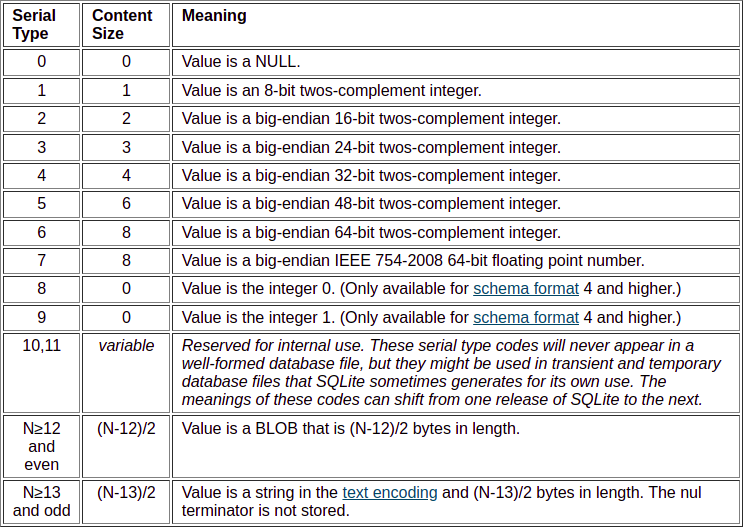
\includegraphics[scale=0.5, ]{assets/serialtypes}}
	\caption{Codici Serial Type}
	\label{fig:serialtypes}
	
\end{figure}

\section{Il formato dei record}
All'interno dell'area contenente i record di ciascuna pagina sono presenti un numero arbitrario di byte utilizzati per memorizzare i record.
\medskip

Ciascun record segue questo formato:
\begin{figure}[ht]
	\centerline{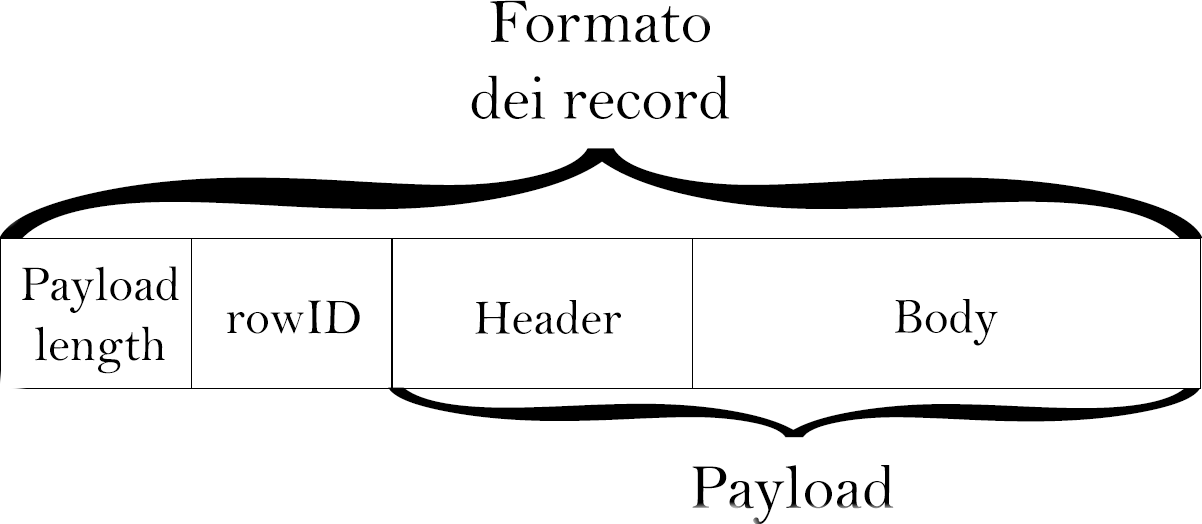
\includegraphics[scale=0.25, ]{assets/record_format}}
	\label{fig:recordformat}
\end{figure}

Per rappresentare questo formato si fa un grande uso delle variabili di tipo varint. 

Il primo campo Payload length, infatti, è rappresentato da una variabile varint che sta a indicare il numero di byte che costituiscono il payload. È presente una seconda variabile varint che memorizza l'id del record. La sezione successiva (payload) memorizza il contenuto delle colonne del record e le informazioni, per risalire al tipo di campo e la lunghezza in byte del contenuto.


\paragraph{Payload}
Questa sezione è a sua volta suddivisa in due sottosezioni: l'header e il body.
Attraverso l'header si è in grado di risalire al numero di campi da cui è composto il record, il tipo di ciascun campo e la dimensione in byte del contenuto.
Queste informazioni sono codificate mediante l'utilizzo del tipo di dato varint e, con l'ausilio dei codici serial types, si riusciranno a identificare i tipi dei campi e la dimensione in byte.
\medskip

Di seguito è presente un'immagine che illustra la struttura dell'header;


\begin{figure}[ht]
	\centerline{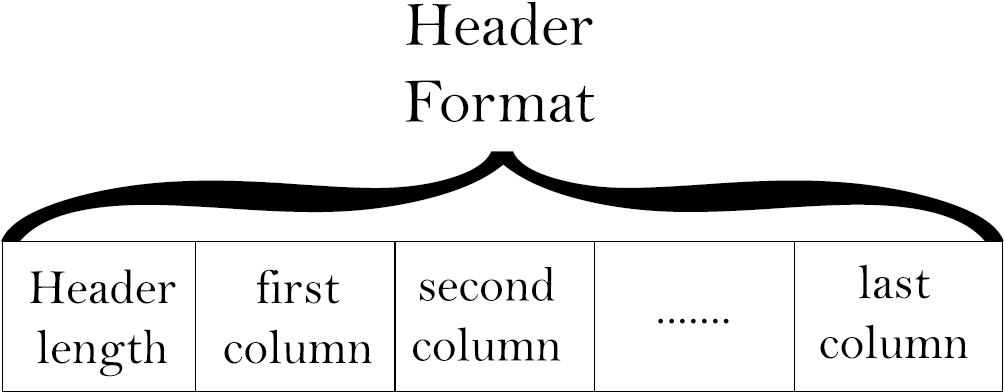
\includegraphics[scale=0.25, ]{assets/record_header_format}}
	\label{fig:recordheaderformat}
\end{figure}

Terminata l'header troviamo il body, all'interno del quale sono presenti diversi byte che ci permettono, sulla base delle informazioni ottenute tramite l'header, di risalire al contenuto del record e quindi dei singoli campi che lo compongono.

\newpage

\paragraph{Esempio}
Per comprendere meglio ciò che è stato precedentemente illustrato, viene presentato un esempio, che, a partire da una sequenza di valori esadecimali rappresentanti un record, ne ricostruisce il contenuto. Questi valori sono stati ottenuti da una pagina foglia di tipo tabella, più precisamente dall'area non allocata.
\medskip

La sequenza di valori presa in esempio è la seguente:

\begin{figure}[ht]
	\centering
	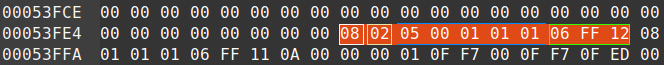
\includegraphics[scale=0.6, ]{assets/hex_record}
	\label{fig:hexrecord}
\end{figure}

Ciascuna sezione che va a comporre il record è contraddistinta da un colore differente.


Ad esclusione dei valori presenti nel body del payload, i restanti sono codificati come variabili di tipo varint. 
Per come viene decodificato questo tipo di dato, i valori minori di 241 vengono convertiti in valori interi come una semplice conversione da esadecimale a intero, per ulteriori informazioni sull'algoritmo utilizzato per codificare e decodificare le variabili varint \cite{varint}.


\begin{itemize}
\item Il primo valore (08) rappresenta il payload length e indica che il payload è composto da 8 byte.
\item Il successivo valore (02) indica che l'id del record è 2. 
\item L'header del payload inizia con il valore 5, che sta a indicare la lughezza in byte dell'header
\item Successivamente troveremo tante variabili varint quante sono le celle che vanno a comporre il record, per ogni variabile varint useremo i codici serial types per ricavarne il tipo e la lunghezza in byte;
\SubItem{Il valore 0 non ci dà informazioni sul tipo della cella, nè della sua lunghezza in byte. Indica solamente che c'è un campo (la row id, di cui abbiamo già il contenuto)}.
\SubItem{Il valore 1 sta a indicare che il contenuto della seconda cella è un numero intero di 8 bit complemento a 2.}
\SubItem{Lo stesso vale per i successivi due valori esadecimali (01 01)}
\item Terminata l'header del payload, troviamo il body evidenziato in verde, tramite questo, e sulla base delle informazioni acquisite dalla sezione precedente, siamo in grado di ottenere il contenuto delle celle.
\SubItem{La seconda cella del record è un intero di 8-bit in ca2, quindi di valore 6}
\SubItem{Lo stesso vale per la terza e quarta cella, cioè -1 (FF) e 18 (12)}
\end{itemize}

\newpage

Ottenute queste informazioni siamo in grado di ricostruire la struttura del record e il contenuto. Ovviamente non possiamo affermare nulla sulla tabella di appartenenza. Vedremo in seguito come poter ottenere un insieme di tabelle potenziali sulla base delle informazioni ottenute dall'header.

\medskip

\begin{figure}[ht]
	\centering
	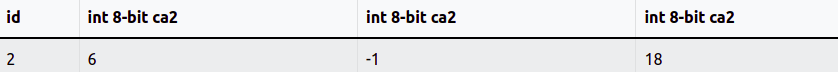
\includegraphics[scale=0.45, ]{assets/record_parse}
	\caption{Record convertito}
	\label{fig:recordparse}
\end{figure}

